\chapter{Giới thiệu}
Mạng nơ ron sâu (DNNs) đã đạt hiệu quả rất tốt với các bài toán trong học máy
và trí tuệ nhân tạo như phân loại ảnh, nhận diện giọng nói, dịch máy và trò chơi.
Mặc dù DNNs rất hiệu quả nhưng mốt số nghiên cứu gần đây đã chứng minh DNNs rất 
dễ  "tổn thương" với các mẫu đối thủ (Szegedy et al. 2013; Goodfellow, Shlens, 
and Szegedy 2015). Ví dụ, một hình ảnh với nhiễu được thiết kế cẩn thận có thể
làm cho một DNNs đã được huấn luyện phân loại sai. Tệ hơn nữa, các mẫu đối thủ
được tạo ra hầu như không thể phân biệt được bằng mắt người. 
\begin{figure}[H] % places figure environment here   
    \centering % Centers Graphic
    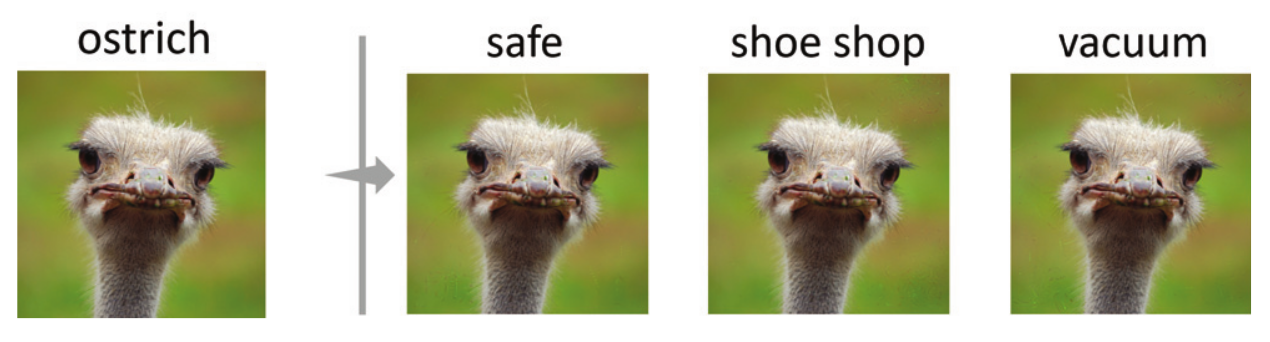
\includegraphics[width=0.8\textwidth]{assets/fig_01.png} 
    \caption{Minh họa trực quan về mẫu đối thủ được sinh bởi EAD. 
    Hình gốc (đà điểu) được lấy từ tập ImageNet. Các mẫu đối thủ bị 
    phân loại sai với mô hình Inception-v3.} % Creates caption underneath graph
    \label{fig:fg_01}
\end{figure}
Ví dụ trực quan trên thể hiện 3 mẫu đối thủ của một hình con đà điểu ("ostrich") 
được sinh ra bằng thuật toán của chúng tôi. Các mẫu này được mô hình Inception-v3 
(Szegedy et al. 2016) phân loại thành "safe", "shoe shop" và "vacuum". \\

Sự thiếu mạnh mẽ của DNNs thể hiện trước các mẫu đối thủ đã làm dấy lên những lo ngại 
nghiêm trọng về vấn đề bảo mật các ứng dụng, bao gồm nhận dạng tín hiệu giao thông 
và phát hiện phần mềm độc hại. Hơn nữa, vượt ra ngoài không gian kỹ thuật số, 
các nhà nghiên cứu đã chỉ ra rằng những mẫu đối thủ này vẫn có hiệu quả trong thế giới 
vật chất trong việc đánh lừa DNNs (Kurakin, Goodfellow, and Bengio 2016a; Evtimov et al. 2017).
Do tính mạnh mẽ và ý nghĩa bảo mật, các phương tiện tạo ra các mẫu đối thủ được gọi là 
các cuộc tấn công (\textit{attacks}) vào DNNs. Cụ thể, các cuộc tấn công có chủ đích 
(\textit{targeted attacks}) nhằm mục đích tạo ra các mẫu đối thủ được phân loại nhầm thành các lớp mục tiêu 
cụ thể và các cuộc tấn công không có mục tiêu (\textit{untargeted attacks}) nhằm mục đích 
để tạo ra các mẫu đối thủ không được phân loại như lớp học ban đầu. Các cuộc tấn công 
chuyển giao (\textit{transfer attacks}) nhằm mục đích tạo ra các mẫu đối thủ có thể chuyển 
từ mô hình DNN này sang mô hình DNN khác. Ngoài việc đánh giá mức độ mạnh mẽ của DNNs,
Các mẫu đối thủ có thể được sử dụng để huẩn luyện một mô hình mạnh có khả năng chống chịu 
với những xáo trộn của đối thủ, được gọi là huấn luyện đối thủ (\textit{adverarial training}) 
(Madry et al. 2017). Chúng cũng có được sử dụng để giải thích DNNs (Koh và Liang 2017;
Dong et al. 2017). \\



